% Mini LMS - Rapport de Projet v3
\documentclass[10pt,a4paper]{article}

\usepackage[utf8]{inputenc}
\usepackage[T1]{fontenc}
\usepackage{geometry}
\usepackage{graphicx}
\usepackage{xcolor}
\usepackage{tabularx}
\usepackage{booktabs}
\usepackage{enumitem}
\usepackage{hyperref}
\usepackage{fancyhdr}
\usepackage{titlesec}
\usepackage{tcolorbox}
\usepackage{amssymb}
\usepackage{multicol}
\usepackage{float}
\usepackage{parskip}
\usepackage{lastpage}

% Diagrams live at <project>/diagrams/d2_compiled/. This .tex lives at
% <project>/latex/code/. Tell graphicx where to find the images so the
% \includegraphics calls below stay short.
\graphicspath{{../../diagrams/d2_compiled/}}

\definecolor{brand}{HTML}{4263EB}
\definecolor{brandDark}{HTML}{364FC7}
\definecolor{brandLight}{HTML}{DBE4FF}
\definecolor{accent}{HTML}{0CA678}
\definecolor{darkText}{HTML}{1E293B}
\definecolor{mediumText}{HTML}{475569}
\definecolor{headerGray}{HTML}{374151}
\definecolor{bgLight}{HTML}{F8FAFC}
\definecolor{warnOrange}{HTML}{D97706}

\newcommand{\faCheck}{\textcolor{accent}{\checkmark}}
\newcommand{\faTimes}{\textcolor{red}{$\times$}}

\geometry{top=2cm, bottom=2.5cm, left=2.2cm, right=2.2cm}
\setlength{\parindent}{0pt}
\setlength{\parskip}{3pt}

\hypersetup{colorlinks=true, linkcolor=brand, urlcolor=brand}

\pagestyle{fancy}
\fancyhf{}
\fancyhead[L]{\small\color{headerGray}\textbf{Mini LMS} - Rapport de Projet}
\fancyhead[R]{\small\color{headerGray}Stage Avril 2026}
\fancyfoot[L]{\small\color{headerGray}Latreche - Mini LMS}
\fancyfoot[R]{\small\color{headerGray}Page \thepage\ / \pageref{LastPage}}
\renewcommand{\headrulewidth}{0.6pt}
\renewcommand{\headrule}{\hbox to\headwidth{\color{brand}\leaders\hrule height \headrulewidth\hfill}}
\renewcommand{\footrulewidth}{0.4pt}
\renewcommand{\footrule}{\hbox to\headwidth{\color{brand!40}\leaders\hrule height \footrulewidth\hfill}}

\titleformat{\section}{\Large\bfseries\color{brandDark}}{\thesection.}{0.5em}{}[\vspace{-4pt}{\color{brand}\rule{\textwidth}{1.5pt}}]
\titleformat{\subsection}{\large\bfseries\color{darkText}}{\thesubsection}{0.5em}{}

\tcbuselibrary{skins,breakable}
\newtcolorbox{infobox}[1][]{colback=brandLight!30, colframe=brand, fonttitle=\bfseries\color{white}, title=#1, coltitle=white, colbacktitle=brand, rounded corners, boxrule=0.5pt, left=8pt, right=8pt, top=6pt, bottom=6pt}
\newtcolorbox{techbox}[1][]{colback=bgLight, colframe=headerGray, coltitle=white, fonttitle=\bfseries, title=#1, rounded corners, boxrule=0.4pt, left=8pt, right=8pt, top=6pt, bottom=6pt}
\newtcolorbox{warnbox}[1][]{colback=orange!5, colframe=warnOrange!70, fonttitle=\bfseries\small\color{white}, title=#1, colbacktitle=warnOrange!70, rounded corners, boxrule=0.4pt, left=6pt, right=6pt, top=4pt, bottom=4pt}

\begin{document}

% TITLE PAGE
\begin{titlepage}
\begin{center}
\vspace*{1.5cm}
{\color{brand}\rule{\textwidth}{2pt}}\\[0.8cm]
{\fontsize{32}{38}\selectfont\bfseries\color{brandDark} Mini LMS}\\[0.3cm]
{\Large\color{mediumText} Plateforme LMS avec G\'en\'eration IA et R\'evision Espac\'ee}\\[0.3cm]
{\color{brand}\rule{8cm}{1pt}}
\vspace{1.2cm}
{\large\color{darkText}
\renewcommand{\arraystretch}{1.6}
\begin{tabular}{r@{\hspace{0.6cm}}l}
\textbf{Stagiaire} & Latreche \\
\textbf{P\'eriode} & Avril 2026 \\
\textbf{Stack} & Laravel 11 \textperiodcentered\ MySQL \textperiodcentered\ Tailwind \textperiodcentered\ Alpine.js \textperiodcentered\ Gemini AI \\
\textbf{Production} & \url{https://latreche-lms.alwaysdata.net} \\
\end{tabular}}
\vspace{1.5cm}
\begin{infobox}[R\'esum\'e]
Plateforme LMS Laravel 11 avec g\'en\'eration de contenu p\'edagogique structur\'e par IA (Gemini), syst\`eme de flashcards avec algorithme de r\'evision espac\'ee SM-2, enrichissement automatique multi-sources (images Wikimedia/Pexels, sources valid\'ees, diagrammes Mermaid) et saisie vocale. Architecture en couches avec autorisation par Policies, isolation stricte des r\^oles, et gestion d'erreurs ind\'ependante du layout dashboard. D\'eploy\'ee sur AlwaysData.
\end{infobox}
\vfill
{\color{brand}\rule{\textwidth}{2pt}}
\end{center}
\end{titlepage}

\tableofcontents
\thispagestyle{empty}
\newpage
\setcounter{page}{1}

% ==========================================
\section{Contexte et Objectifs}
% ==========================================

\subsection{Contexte}
Concevoir une plateforme LMS exploitant l'IA g\'en\'erative pour la cr\'eation automatique de contenu p\'edagogique structur\'e (formations, chapitres, quiz, flashcards), avec une isolation stricte entre r\^oles et un syst\`eme de r\'evision espac\'ee.

\subsection{Objectifs}
\begin{table}[H]
\centering\renewcommand{\arraystretch}{1.3}
\begin{tabularx}{\textwidth}{>{\centering\arraybackslash}p{0.5cm} X >{\centering\arraybackslash}p{1.5cm}}
\toprule \textbf{\#} & \textbf{Objectif} & \textbf{Statut} \\ \midrule
1 & Architecture Laravel en couches (Service Layer + Policies + FormRequests) & \faCheck \\
2 & Authentification multi-r\^oles avec redirection bas\'ee sur le r\^ole et isolation stricte des layouts & \faCheck \\
3 & Quiz step-by-step avec scoring s\'ecuris\'e (anti-triche, verrou pessimiste) & \faCheck \\
4 & Flashcards avec algorithme SM-2 et distribution automatique sur inscription & \faCheck \\
5 & G\'en\'eration IA contr\^ol\'ee : nombre de chapitres, profondeur, type, fichiers joints & \faCheck \\
6 & Pipeline d'enrichissement multi-sources avec fallbacks (images, sources, diagrammes) & \faCheck \\
7 & Parit\'e d'\'edition admin/\'etudiant pour les formations g\'en\'er\'ees par l'\'etudiant & \faCheck \\
8 & D\'eploiement production sur h\'ebergement mutualis\'e & \faCheck \\
\bottomrule
\end{tabularx}
\end{table}

% ==========================================
\section{Stack Technique}
% ==========================================

\begin{table}[H]
\centering\renewcommand{\arraystretch}{1.3}
\begin{tabularx}{\textwidth}{p{2.5cm} p{3.2cm} X}
\toprule \textbf{Couche} & \textbf{Technologie} & \textbf{Justification} \\ \midrule
Backend & Laravel 11, PHP 8.2 & Eloquent, migrations, policies, FormRequests \\
BDD & MySQL 8 / SQLite & MySQL prod, SQLite dev local \\
Frontend & Blade + Tailwind CDN & Server-rendered, pas de build step \\
Interactivit\'e & Alpine.js & Quiz step-by-step, modales, formulaires r\'eactifs \\
Diagrammes & Mermaid.js (CDN) & Rendu client-side du code IA, \texttt{securityLevel: strict} \\
Voix & Web Speech API & Saisie native FR/EN/AR, sans backend \\
IA & Google Gemini API & JSON structur\'e, multi-mod\`ele fallback, Files API \\
Images & Wikimedia + Pexels & CC en priorit\'e, fallback paysage \\
H\'ebergement & AlwaysData & PHP/MySQL mutualis\'e \\
\bottomrule
\end{tabularx}
\end{table}

% ==========================================
\section{Architecture}
% ==========================================

\subsection{Flux de requ\^ete}
\begin{center}
\texttt{Request \textrightarrow\ Auth+Role MW \textrightarrow\ FormRequest \textrightarrow\ Controller \textrightarrow\ Service \textrightarrow\ Model \textrightarrow\ DB}
\end{center}

Les contr\^oleurs sont \emph{thin} : orchestration uniquement (validation d\'el\'egu\'ee aux \texttt{FormRequest}, autorisation aux \texttt{Policies}, logique m\'etier aux \texttt{Services}). Tout 403/404/500 est rendu via \texttt{layouts.error} (layout d\'edi\'e, sans sidebar) pour qu'aucune erreur ne fuite la chrome du r\^ole oppos\'e.

\begin{figure}[H]
\centering
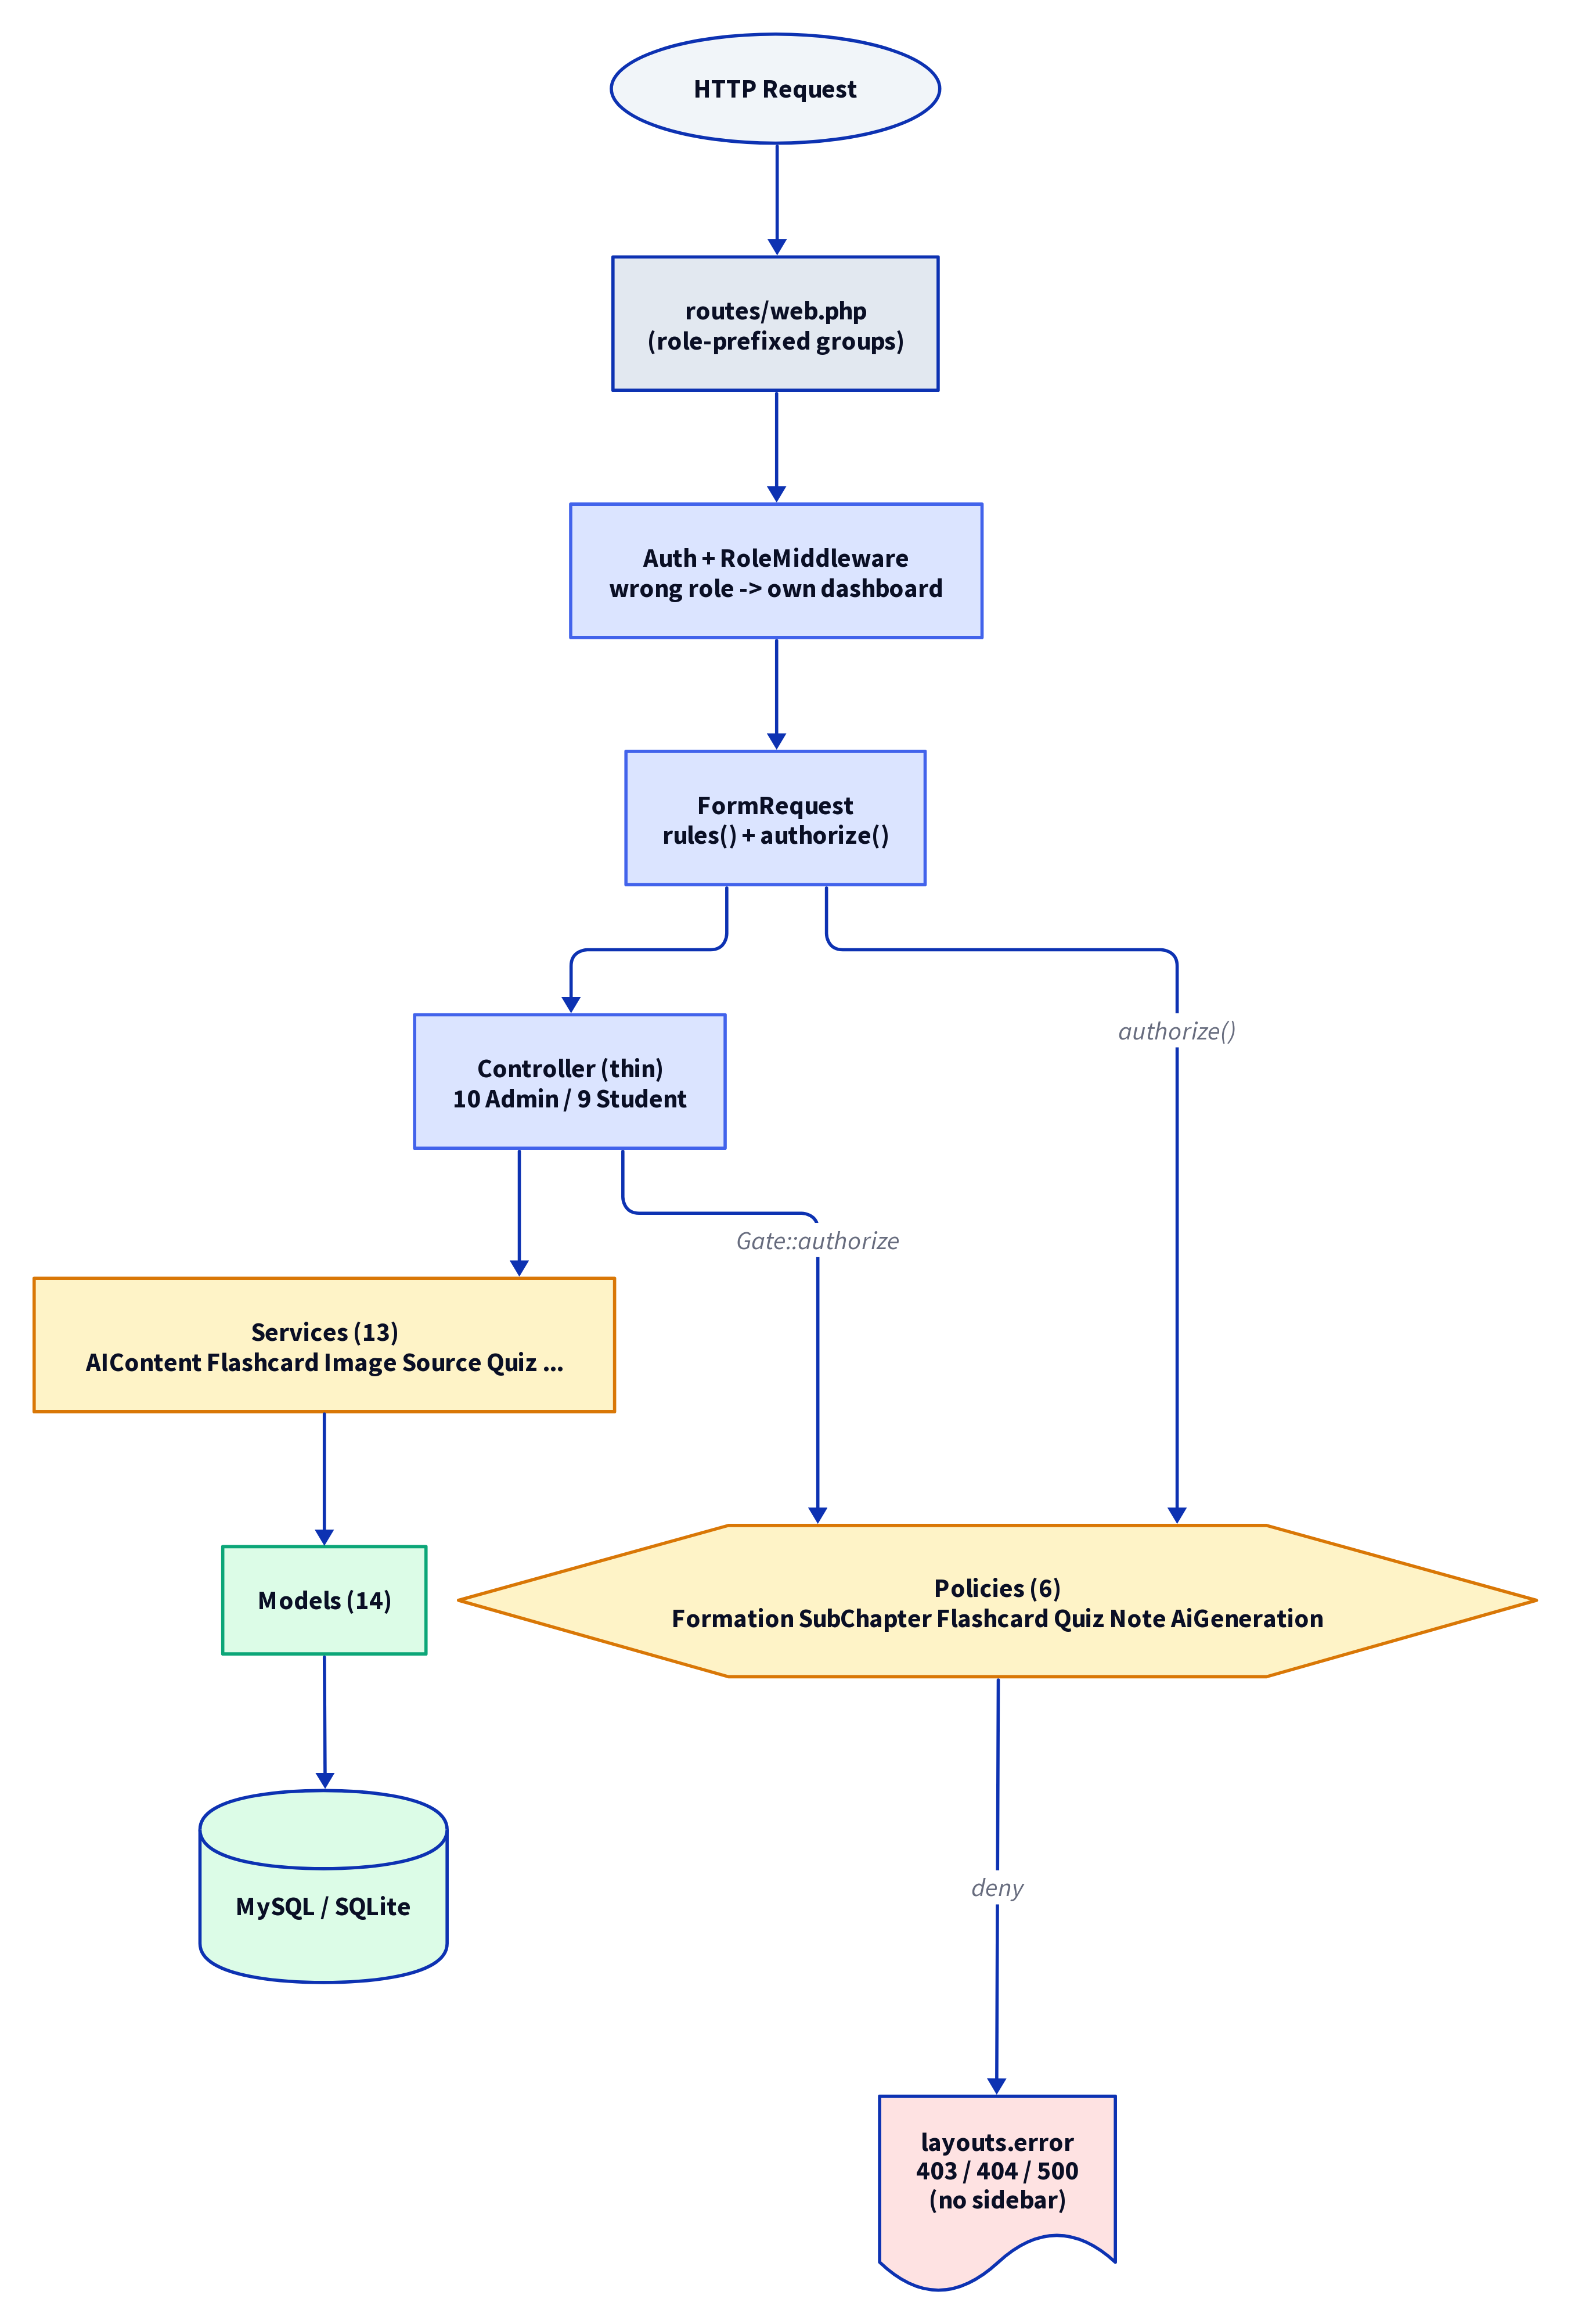
\includegraphics[width=0.85\textwidth]{archi.png}
\caption{Architecture en couches : isolation des responsabilit\'es, policies en garde sur chaque action sensible}
\label{fig:archi}
\end{figure}

\subsection{Inventaire des composants}
\begin{table}[H]
\centering\renewcommand{\arraystretch}{1.3}
\begin{tabularx}{\textwidth}{p{4.5cm} >{\centering\arraybackslash}p{1.2cm} X}
\toprule \textbf{Composant} & \textbf{N} & \textbf{R\^ole} \\ \midrule
Controllers Admin & 10 & CRUD complet : formations, chapitres, sous-chapitres, quizzes, questions, users, notes, AI, flashcards \\
Controllers Student & 9 & Lecture + CRUD sur formations \emph{poss\'ed\'ees}, AI, flashcards, todos \\
\texttt{AuthController} & 1 & Login/register/logout, redirection par r\^ole \\
FormRequests & 9 & Validation + \texttt{authorize()} bas\'ee sur les Policies \\
Policies & 6 & \texttt{Formation}, \texttt{SubChapter}, \texttt{Flashcard}, \texttt{Quiz}, \texttt{Note}, \texttt{AiGeneration} \\
Models Eloquent & 14 & Avec relations, scopes, casts, soft deletes \\
Services & 13 & Logique m\'etier, transactions, APIs externes (voir \S\ref{sec:enrichment}) \\
Migrations & 16 & Sch\'ema + colonnes enrichissement + flashcards + ownership + CHECK \texttt{type='full'} \\
Vues Blade & 60+ & Layouts (\texttt{app}, \texttt{error}), partials, vues admin/student \\
\bottomrule
\end{tabularx}
\end{table}

% ==========================================
\section{Mod\`ele de Donn\'ees}
% ==========================================

\begin{figure}[H]
\centering
\includegraphics[width=\textwidth]{erd.png}
\caption{ERD : 14 entit\'es principales (+ tables auxiliaires regroup\'ees), enrichissement IA sur \texttt{chapters} et \texttt{sub\_chapters}, soft delete sur formations, ownership via \texttt{created\_by}}
\label{fig:erd}
\end{figure}

\subsection{Colonnes cl\'es}
\begin{table}[H]
\centering\renewcommand{\arraystretch}{1.3}
\begin{tabularx}{\textwidth}{p{3.2cm} p{3.5cm} X}
\toprule \textbf{Colonne} & \textbf{Tables} & \textbf{Usage} \\ \midrule
\texttt{image\_url}, \texttt{image\_credit} & chapters, sub\_chapters & Image illustrative + attribution licence \\
\texttt{sources} (JSON) & chapters, sub\_chapters & Tableau \{title, url, type\} valid\'e \\
\texttt{mermaid\_code} (TEXT) & chapters, sub\_chapters & Diagramme g\'en\'er\'e par IA \\
\texttt{created\_by} & formations & Trace l'auteur (admin ou \'etudiant) pour ownership \\
\texttt{type} CHECK & ai\_generations & \texttt{course} \textbar\ \texttt{quiz} \textbar\ \texttt{mixed} \textbar\ \texttt{full} (cours+quiz+flashcards) \\
\texttt{is\_template} & flashcards & S\'epare cartes de distribution (admin) et cartes \'etudiables (SM-2) \\
\texttt{ease\_factor}, \texttt{interval\_days}, \texttt{next\_review\_at} & flashcards & \'Etat SM-2 par carte \'etudiable \\
\texttt{validated\_at} & ai\_generations & Marqueur de validation par l'\'etudiant \\
\bottomrule
\end{tabularx}
\end{table}

% ==========================================
\section{Authentification \& Redirection par R\^ole}
% ==========================================

Le syst\`eme d'authentification a \'et\'e con\c{c}u pour \'eviter le bug classique de redirection inter-r\^oles : un admin dont la session expire sur \texttt{/admin/...}, suivi d'une connexion \'etudiant, ne doit \emph{jamais} se voir redirig\'e vers une URL admin et obtenir un 403 \emph{dans le layout admin}.

\begin{figure}[H]
\centering
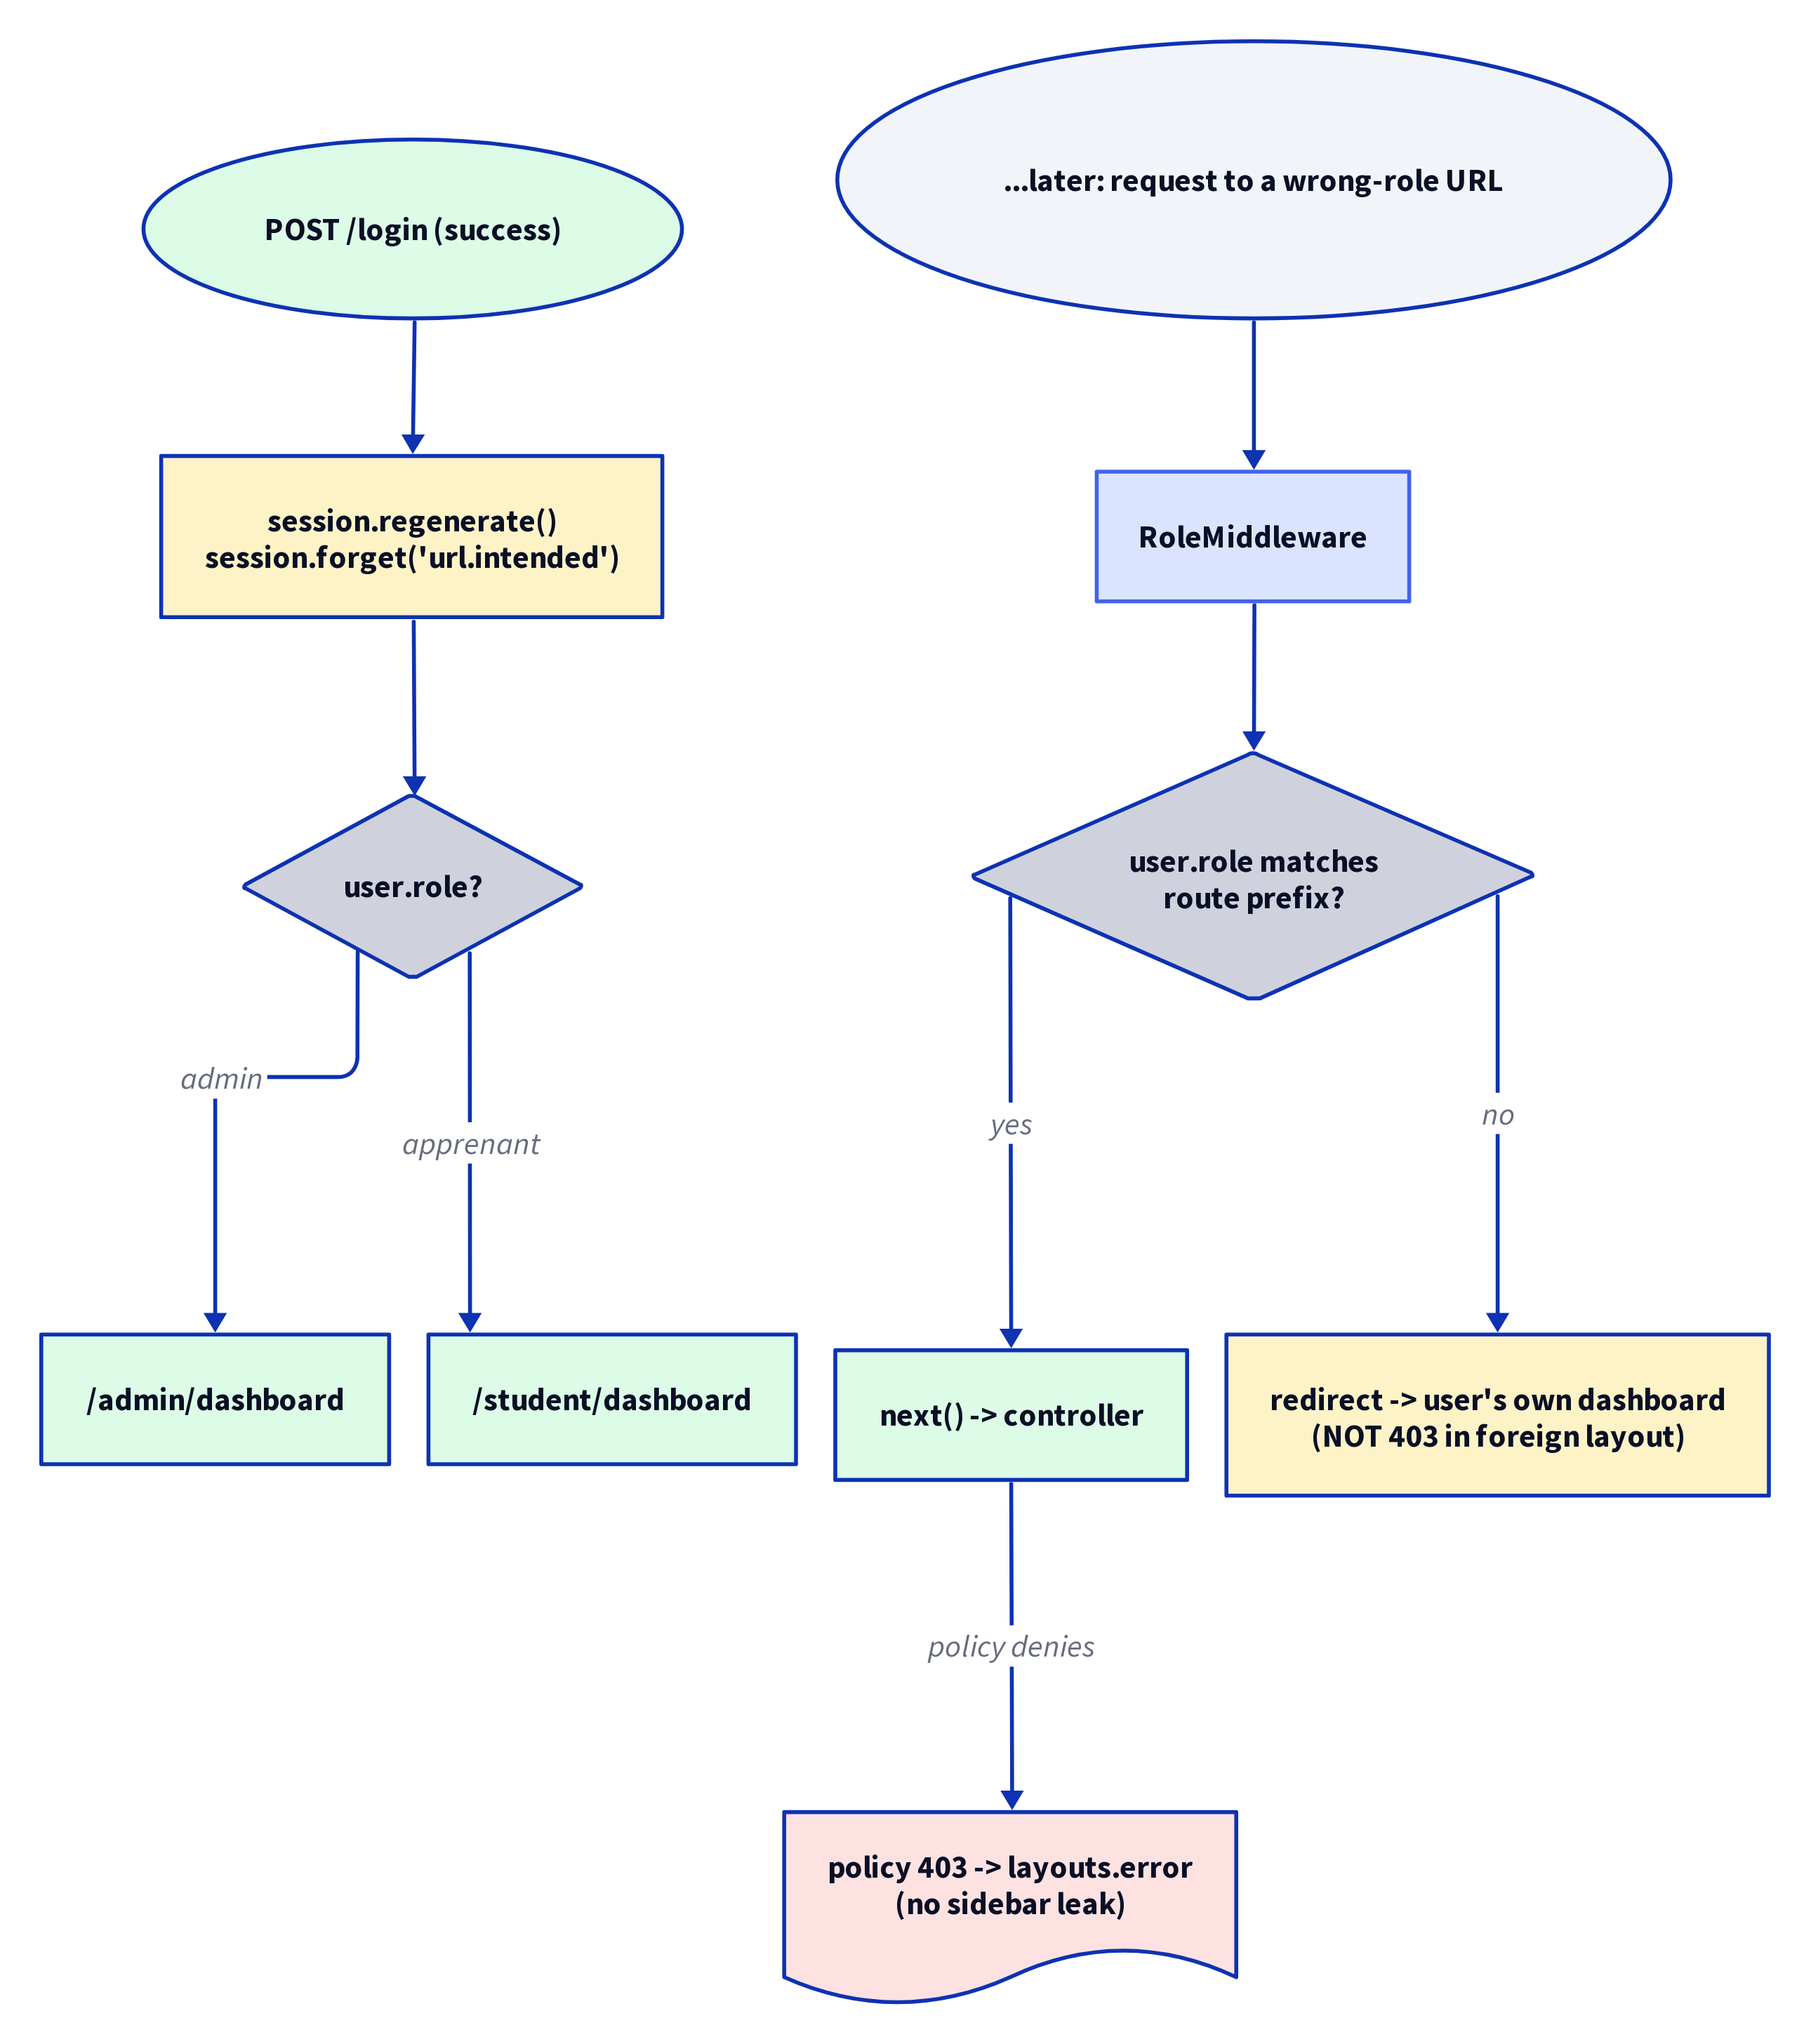
\includegraphics[width=\textwidth]{auth.png}
\caption{Flux de login + RoleMiddleware : la redirection est pilot\'ee strictement par \texttt{user.role}, jamais par \texttt{intended()}}
\label{fig:auth}
\end{figure}

\subsection{Insights cl\'es}
\begin{itemize}[leftmargin=*, itemsep=2pt]
  \item \textbf{Pas d'\texttt{intended()} URL} : \texttt{AuthController::login} appelle \texttt{forget('url.intended')} avant de rediriger, supprimant la cause racine du bug inter-r\^oles.
  \item \textbf{\texttt{RoleMiddleware} redirige plut\^ot que d'abort 403} : un \'etudiant qui touche une URL admin est redirig\'e vers \emph{son} dashboard, pas trait\'e par un 403 dans le layout admin.
  \item \textbf{Layout d'erreur d\'edi\'e} : si un 403 doit malgr\'e tout appara\^itre (apr\`es un \texttt{Gate::authorize}), il s'affiche dans \texttt{layouts.error} (sans sidebar, sans chrome de r\^ole).
  \item \textbf{Session r\'eg\'en\'er\'ee} \`a chaque login pour pr\'evenir la fixation.
\end{itemize}

% ==========================================
\section{R\^oles \& Permissions}
% ==========================================

\begin{table}[H]
\centering\renewcommand{\arraystretch}{1.3}
\begin{tabularx}{\textwidth}{X c c}
\toprule \textbf{Action} & \textbf{Admin} & \textbf{Apprenant} \\ \midrule
Tableau de bord (m\'etriques) & \faCheck & \faCheck \\
CRUD formations / chapitres / sous-chapitres officiels & \faCheck & \faTimes \\
CRUD complet sur formations \emph{g\'en\'er\'ees par soi-m\^eme} & --- & \faCheck \\
Inscription des apprenants \`a une formation & \faCheck & \faTimes \\
Consultation formations enroll\'ees / publi\'ees & \faCheck & \faCheck \\
Quiz step-by-step + scoring & \faTimes & \faCheck \\
G\'en\'eration de quiz sur sous-chapitre existant & \faCheck & \faTimes \\
Notes /20 (administration) & \faCheck & \faCheck (lecture) \\
Notes personnelles par sous-chapitre & \faTimes & \faCheck \\
Todos personnelles & \faTimes & \faCheck \\
Flashcards : templates (distribu\'es \`a l'inscription) & \faCheck & \faTimes \\
Flashcards : copies personnelles \'etudiables (SM-2) & \faCheck & \faCheck \\
G\'en\'eration IA \textrightarrow\ import en formation officielle & \faCheck & \faTimes \\
G\'en\'eration IA \textrightarrow\ validation en formation personnelle & \faTimes & \faCheck \\
\bottomrule
\end{tabularx}
\end{table}

\textbf{Ownership} : \texttt{formations.created\_by} trace l'auteur. La parit\'e d'\'edition de l'\'etudiant repose sur \texttt{FormationPolicy::update} et \texttt{SubChapterPolicy::update}, qui retournent \texttt{true} ssi le user est l'auteur. Les boutons d'\'edition appara\^issent via \texttt{auth()->user()->can('update', \$model)}, jamais par v\'erification de r\^ole.

\textbf{S\'ecurit\'e quiz} : la g\'en\'eration de quiz sur un sous-chapitre est r\'eserv\'ee \`a l'admin. Un \texttt{Quiz} est li\'e 1:1 au \texttt{SubChapter}, donc un quiz cr\'e\'e par un \'etudiant sur un sous-chapitre admin serait visible par tous les autres \'etudiants inscrits — comportement intentionnellement bloqu\'e.

% ==========================================
\section{Flashcards (R\'evision Espac\'ee SM-2)}
% ==========================================

\begin{figure}[H]
\centering
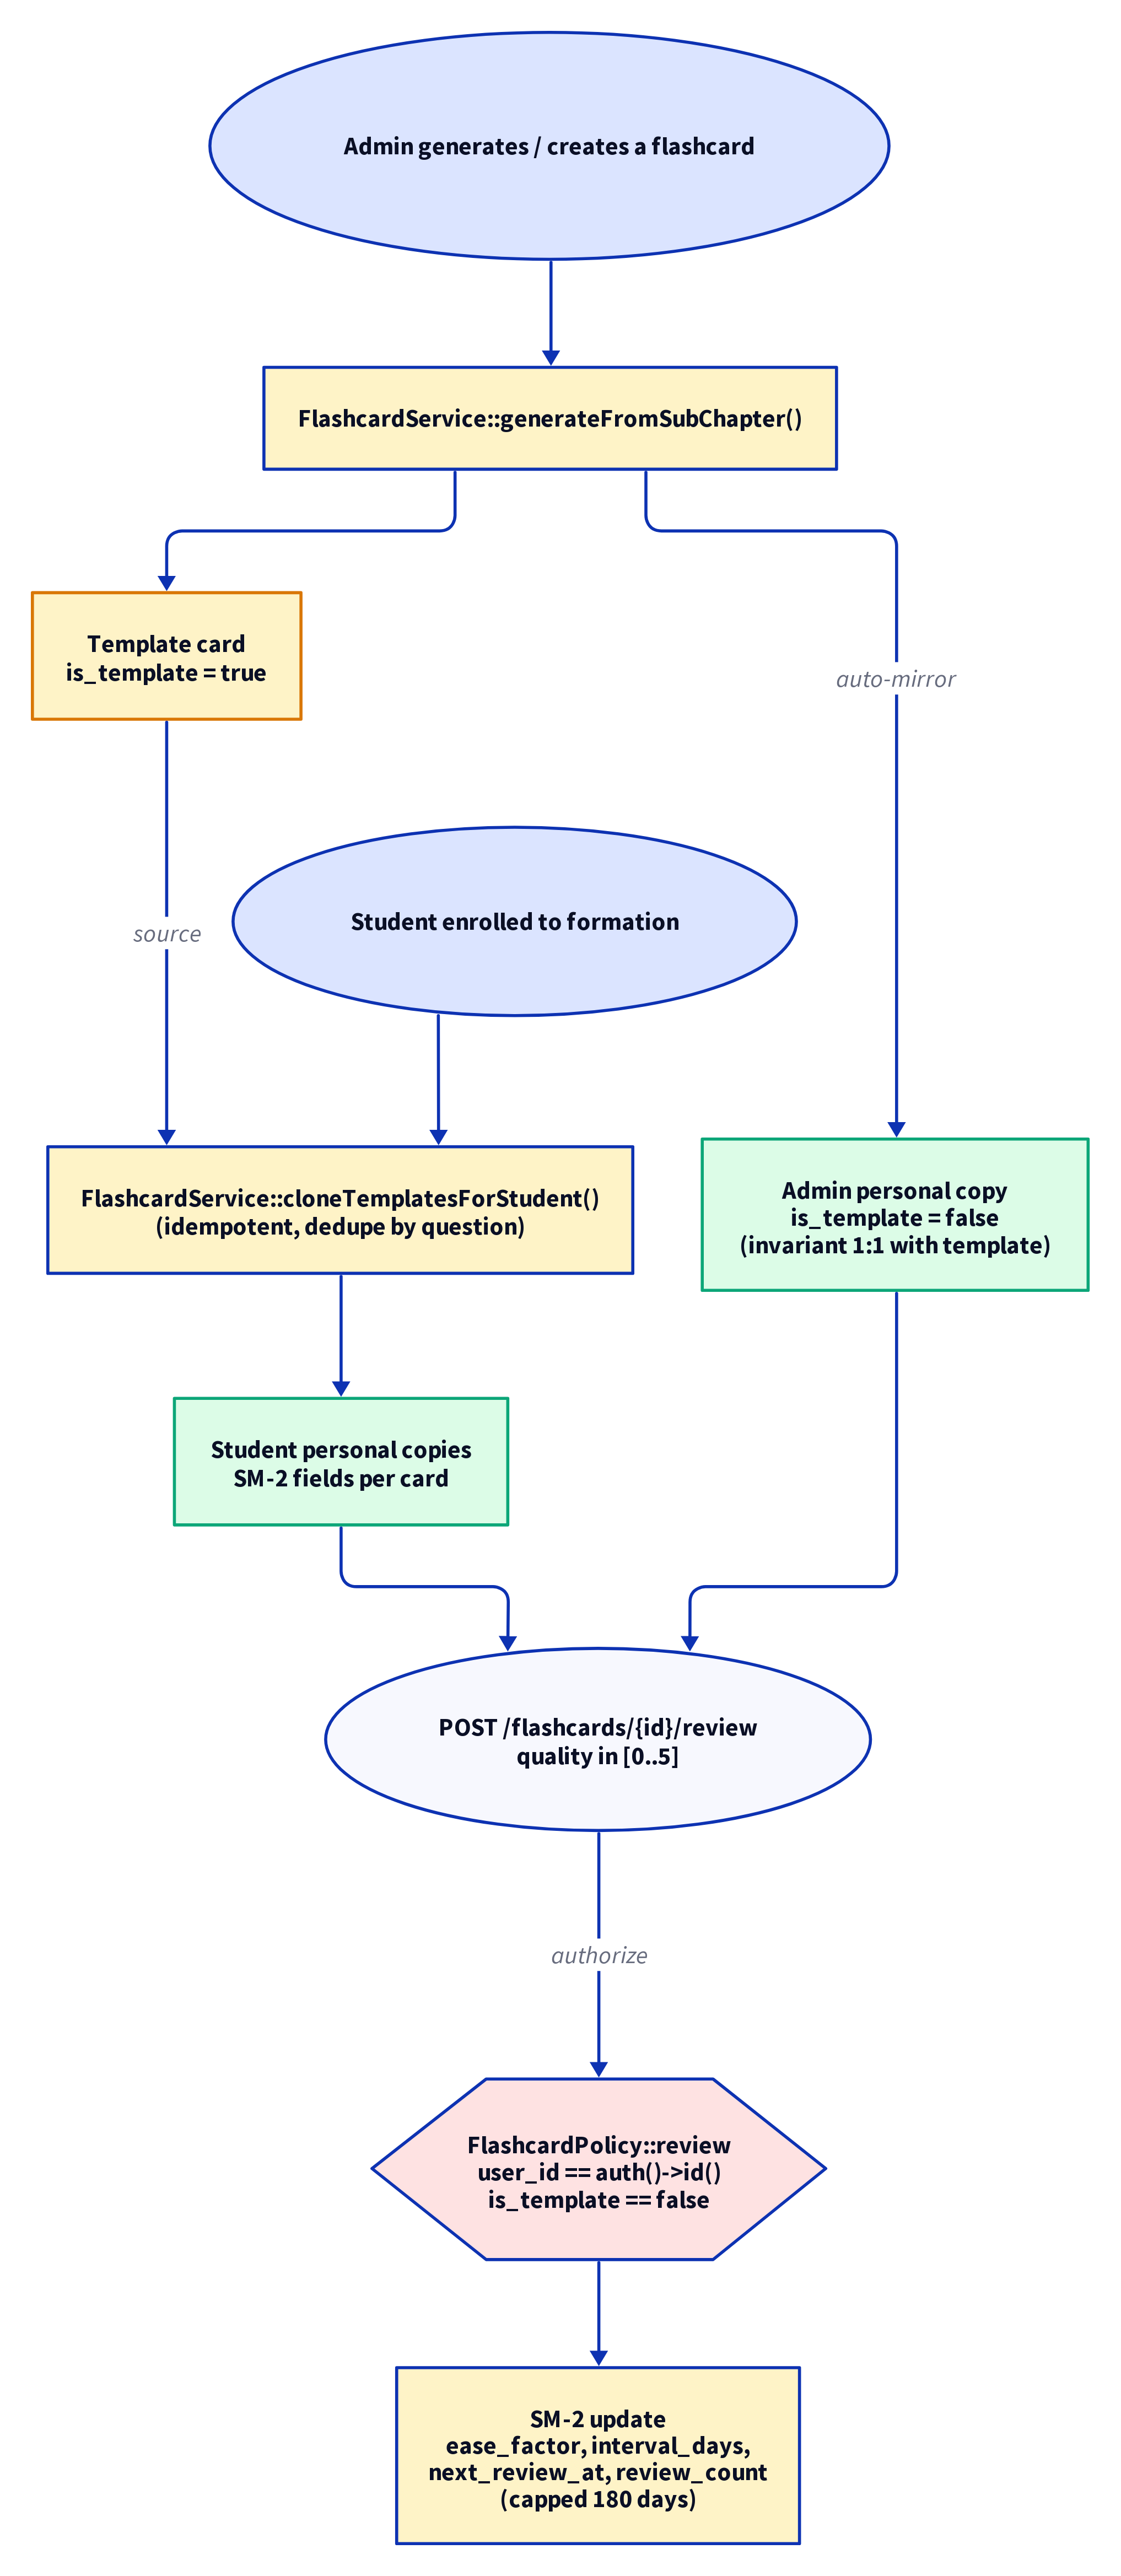
\includegraphics[width=0.6\textwidth]{flashcards.png}
\caption{Mod\`ele dual templates / personnelles, clonage automatique \`a l'inscription, mise \`a jour SM-2 \`a chaque r\'evision}
\label{fig:flashcards}
\end{figure}

\subsection{Insights cl\'es}
\begin{itemize}[leftmargin=*, itemsep=2pt]
  \item \textbf{Deux types de cartes} via \texttt{is\_template} : les \emph{templates} (admin) ne sont pas \'etudiables ; les copies \emph{personnelles} portent l'\'etat SM-2 complet.
  \item \textbf{Invariant admin} : pour chaque template d\'etenu par un admin, il existe une copie personnelle par le m\^eme admin (garantie par \texttt{FlashcardService} \`a chaque entr\'ee : \texttt{generate}, \texttt{store}, \texttt{update}, \texttt{destroy}). Cons\'equence : le mode \emph{Test} de l'admin fonctionne toujours.
  \item \textbf{Distribution \`a l'inscription} : \texttt{cloneTemplatesForStudent()} duplique les templates en copies personnelles, idempotent (d\'edupe par question).
  \item \textbf{SM-2 standard} : \texttt{quality} 0-5, mise \`a jour de \texttt{ease\_factor}, \texttt{interval\_days}, \texttt{next\_review\_at}, \texttt{review\_count}. Intervalle plafonn\'e \`a 180 jours.
  \item \textbf{Politique stricte} : \texttt{FlashcardPolicy::review} exige \texttt{user\_id === auth()->id()} et \texttt{is\_template === false} ; aucun risque d'IDOR cross-user ou d'\'etude des templates.
\end{itemize}

% ==========================================
\section{Module IA - G\'en\'eration de Contenu}
% ==========================================

\subsection{Pipeline}
\begin{figure}[H]
\centering
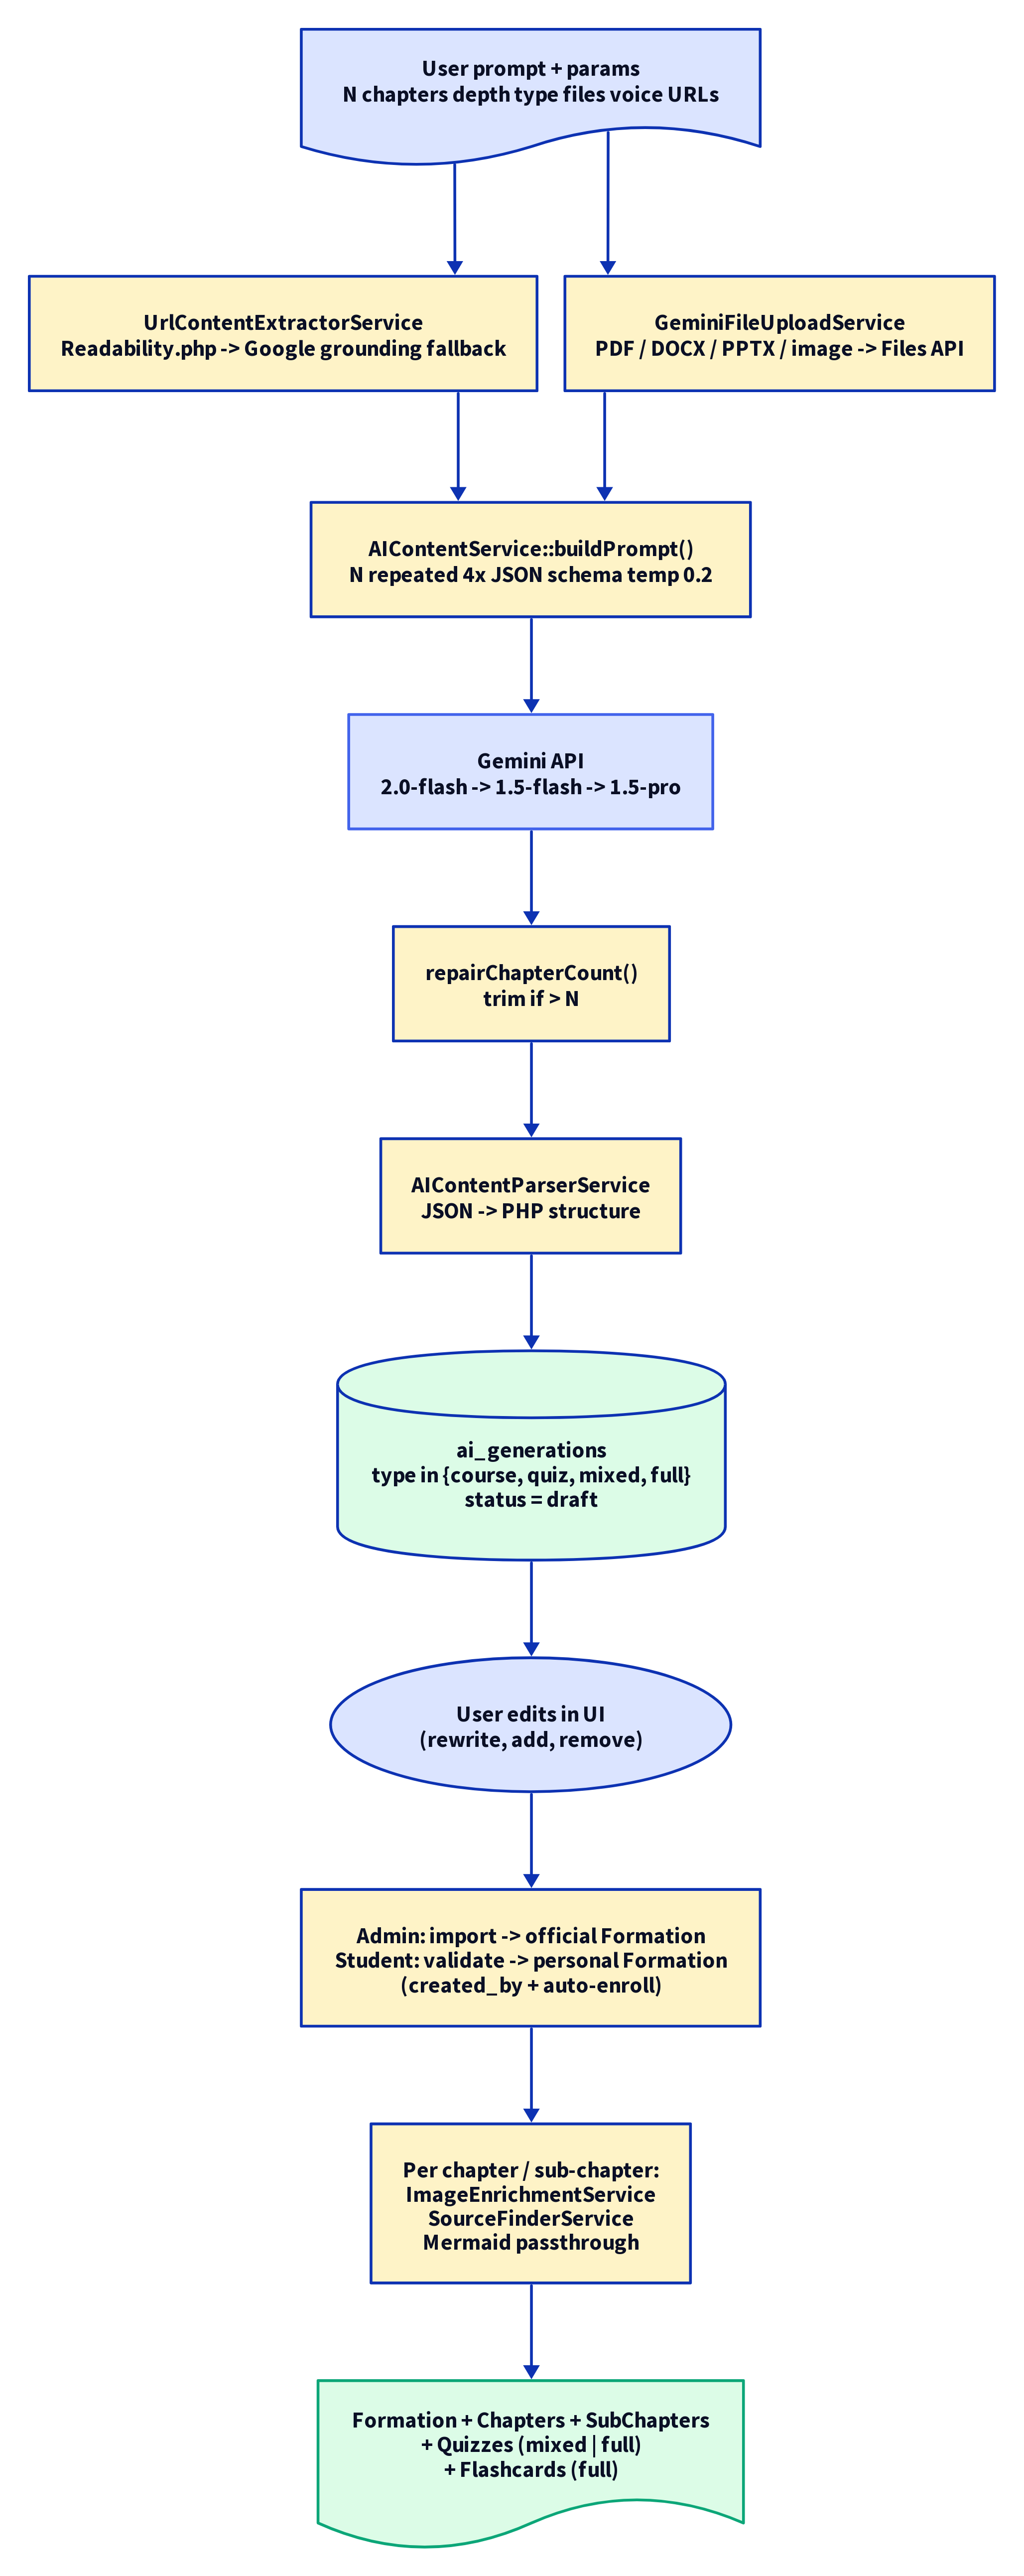
\includegraphics[width=0.55\textwidth]{ai.png}
\caption{Pipeline complet : prompt \textrightarrow\ extraction URL/fichiers \textrightarrow\ Gemini \textrightarrow\ r\'eparation \textrightarrow\ \'edition \textrightarrow\ import enrichi}
\label{fig:ai}
\end{figure}

\subsection{Param\`etres}
\begin{table}[H]
\centering\renewcommand{\arraystretch}{1.3}
\begin{tabularx}{\textwidth}{p{3.5cm} X}
\toprule \textbf{Param\`etre} & \textbf{D\'etail} \\ \midrule
Mod\`eles fallback & \texttt{gemini-2.0-flash} \textrightarrow\ \texttt{1.5-flash} \textrightarrow\ \texttt{1.5-pro} \\
Temp\'erature & 0.2 (instruction-following), 0.3 (flashcards), 0.4 (rewrite) \\
Nombre de chapitres & 1-10 ; r\'ep\'et\'e 4\textperiodcentered\ dans le prompt + \texttt{repairChapterCount()} post-trim \\
Profondeur & Standard (\textasciitilde 300 mots), D\'etaill\'e (\textasciitilde 600), Exhaustif (1000+) par sous-chapitre \\
Type & \texttt{course}, \texttt{quiz}, \texttt{mixed}, \texttt{full} (cours + quiz + flashcards \`a l'import) \\
Pi\`eces jointes & 5 max, 25\,Mo total (PDF, DOCX, PPTX, images), via Gemini Files API \\
URLs & D\'etection auto, extraction Readability.php, fallback Google Search Grounding \\
Saisie vocale & Web Speech API (FR/EN/AR), append au textarea \\
Output & JSON forc\'e (\texttt{responseMimeType}), 40000 tokens max \\
\bottomrule
\end{tabularx}
\end{table}

\subsection{Type \texttt{full} (cours + quiz + flashcards)}

Le type \texttt{full} est un \emph{marqueur} sur \texttt{ai\_generations.type} : la g\'en\'eration produit du contenu \texttt{mixed} (cours + quiz), puis l'enregistrement est promu \`a \texttt{full} pour signaler \`a l'importeur de g\'en\'erer aussi des flashcards pour chaque sous-chapitre. La contrainte CHECK SQLite (\texttt{type IN \{course, quiz, mixed, full\}}) a \'et\'e \'etendue par migration d\'edi\'ee pour autoriser cette promotion.

\subsection{Contr\^ole du nombre de chapitres}
\begin{table}[H]
\centering\renewcommand{\arraystretch}{1.3}
\begin{tabularx}{\textwidth}{>{\centering\arraybackslash}p{0.5cm} p{3.5cm} X}
\toprule \textbf{\#} & \textbf{M\'ecanisme} & \textbf{R\^ole} \\ \midrule
1 & Prompt unifi\'e & Suppression du split system/user \\
2 & R\'ep\'etition 4\textperiodcentered & N rappel\'e dans r\`egles, schema, exemple, footer \\
3 & Temp\'erature 0.2 & Conformit\'e \textgreater\ cr\'eativit\'e \\
4 & JSON mode forc\'e & \texttt{responseMimeType: application/json} \\
5 & R\'eparation post-gen & \texttt{count(chapters) \textgreater\ N} \textrightarrow\ trim \`a N \\
\bottomrule
\end{tabularx}
\end{table}

\subsection{Workflow par r\^ole}
\begin{table}[H]
\centering\renewcommand{\arraystretch}{1.3}
\begin{tabularx}{\textwidth}{p{2cm} X}
\toprule \textbf{R\^ole} & \textbf{Transitions} \\ \midrule
Admin & \texttt{draft} \textrightarrow\ \'edition \textrightarrow\ \texttt{import} \textrightarrow\ \texttt{published} (Formation officielle, \texttt{created\_by} = admin) \\
Apprenant & \texttt{draft} \textrightarrow\ \'edition \textrightarrow\ \texttt{validate} \textrightarrow\ \texttt{validated} (Formation personnelle, \texttt{created\_by} = \'etudiant, auto-inscription) \\
\bottomrule
\end{tabularx}
\end{table}

% ==========================================
\section{Pipeline d'Enrichissement}
\label{sec:enrichment}
% ==========================================

\begin{figure}[H]
\centering
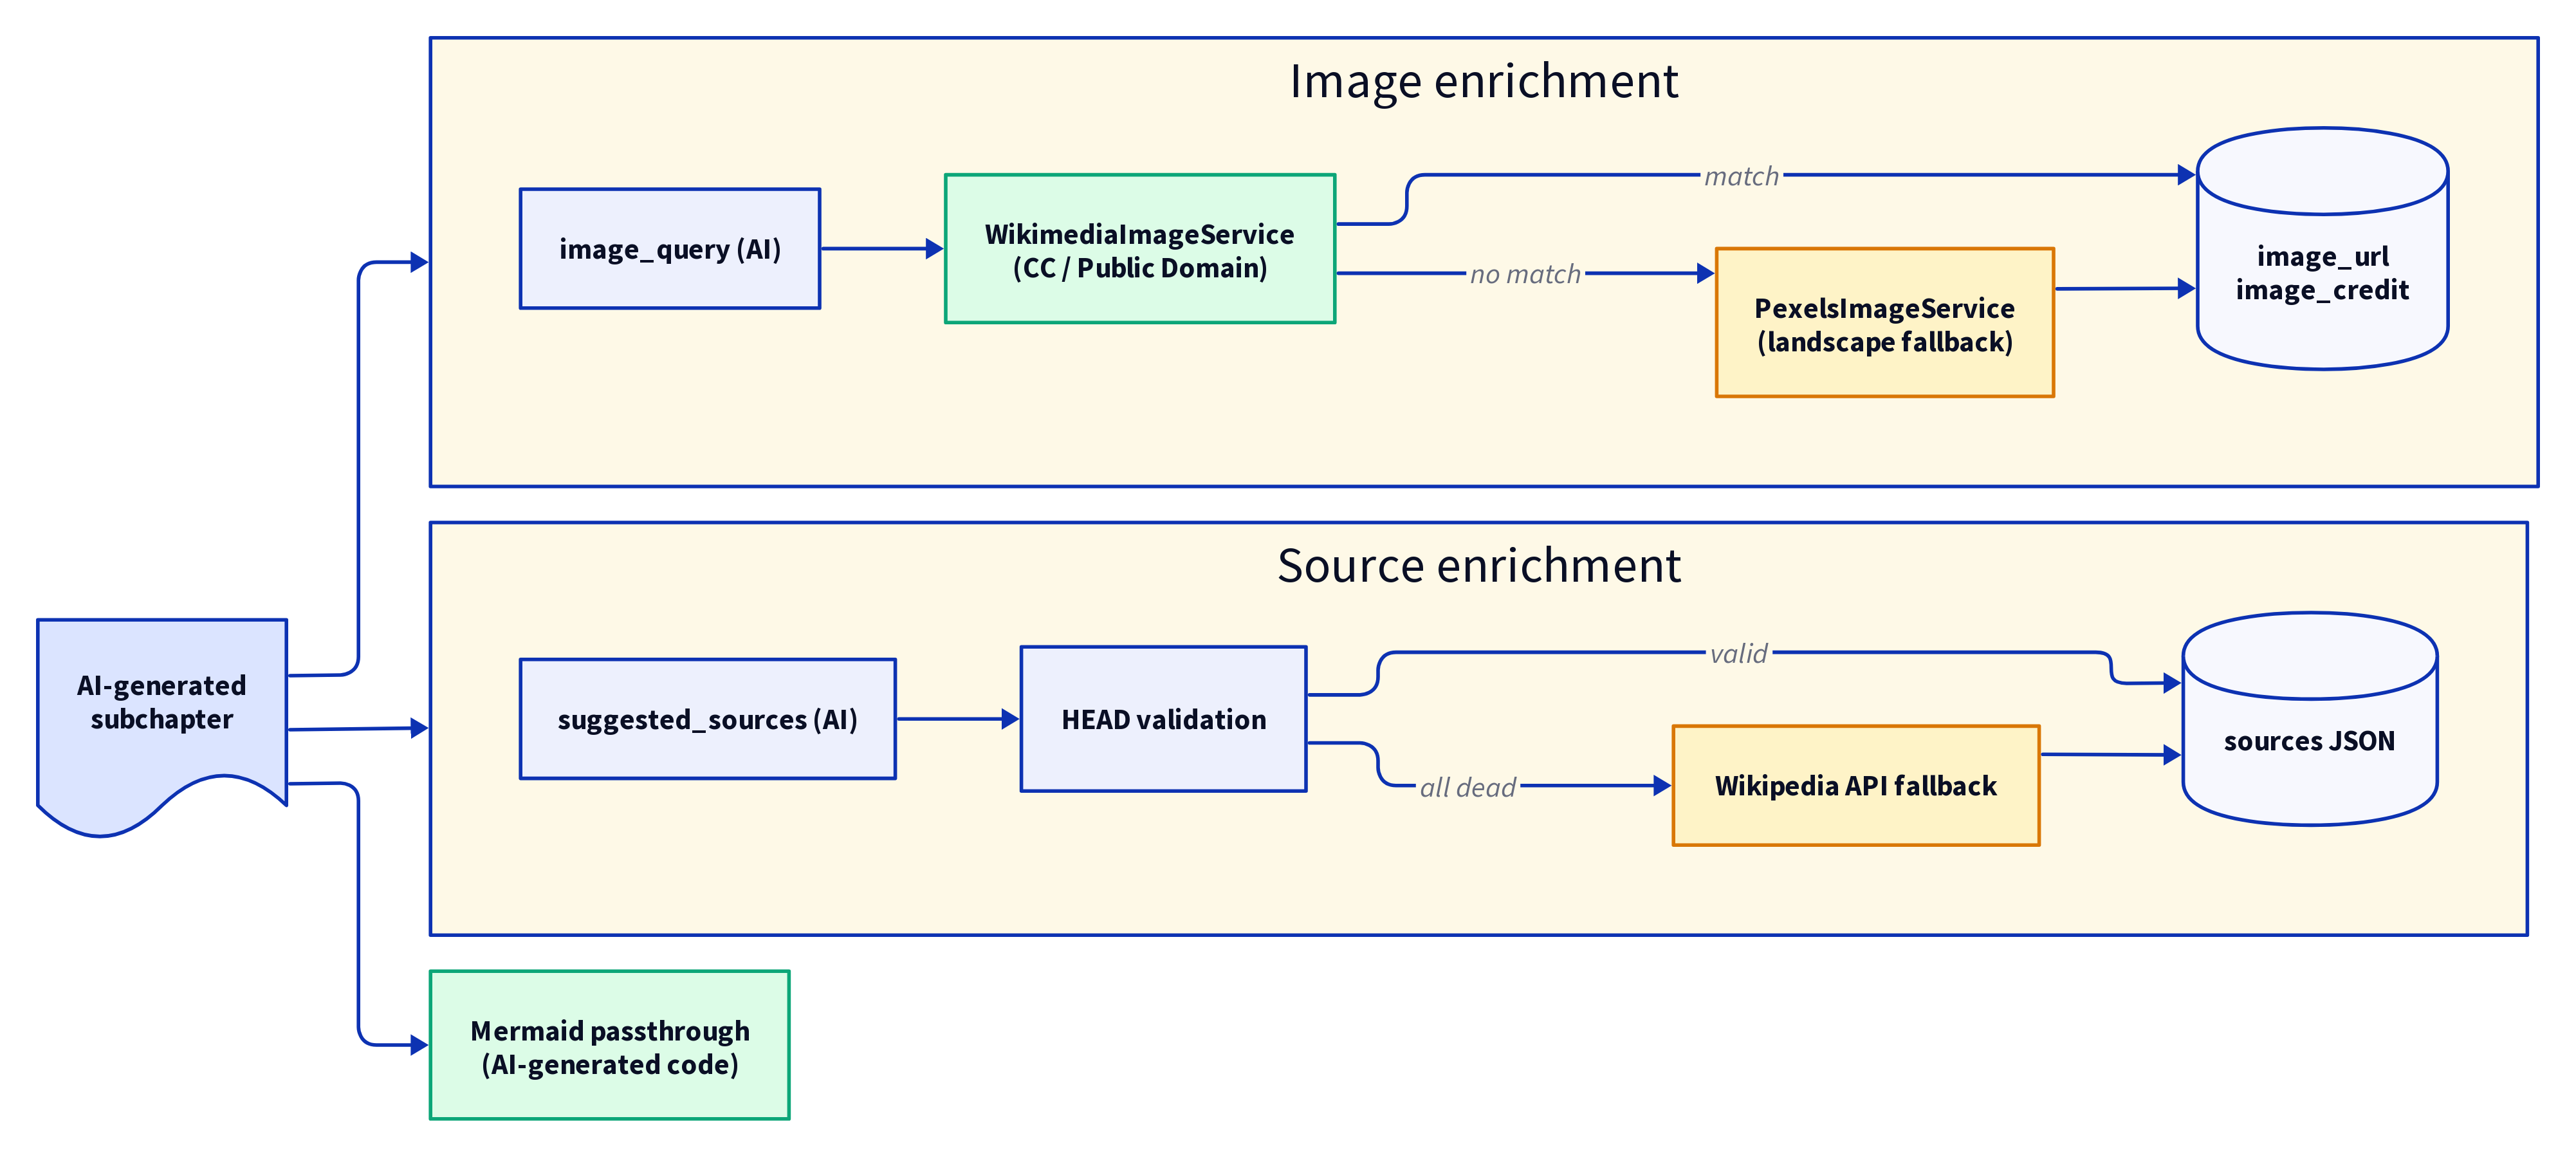
\includegraphics[width=\textwidth]{enrich.png}
\caption{Strat\'egie duale avec fallbacks : images CC en priorit\'e, sources valid\'ees par HEAD, repli Wikipedia}
\label{fig:enrich}
\end{figure}

\begin{table}[H]
\centering\renewcommand{\arraystretch}{1.3}
\begin{tabularx}{\textwidth}{p{2.5cm} p{3cm} p{3cm} X}
\toprule \textbf{\'El\'ement} & \textbf{Source primaire} & \textbf{Fallback} & \textbf{Stockage} \\ \midrule
Images & Wikimedia Commons (CC) & Pexels API & \texttt{image\_url, image\_credit} \\
Sources & IA \texttt{suggested\_sources} valid\'e par HEAD & Wikipedia API par mots-cl\'es & \texttt{sources} JSON \\
Diagrammes & IA Mermaid (passthrough) & --- & \texttt{mermaid\_code} TEXT \\
\bottomrule
\end{tabularx}
\end{table}

\textbf{Services impliqu\'es} (13 au total) : \texttt{AIContentService}, \texttt{AIContentParserService}, \texttt{AIContentImportService}, \texttt{GeminiFileUploadService}, \texttt{UrlContentExtractorService}, \texttt{ImageEnrichmentService}, \texttt{WikimediaImageService}, \texttt{PexelsImageService}, \texttt{SourceFinderService}, \texttt{FlashcardService}, \texttt{QuizService}, \texttt{DashboardService}, \texttt{ContentSanitizer}.

% ==========================================
\section{S\'ecurit\'e}
% ==========================================

\begin{table}[H]
\centering\renewcommand{\arraystretch}{1.3}
\begin{tabularx}{\textwidth}{p{3cm} X}
\toprule \textbf{Menace} & \textbf{Protection} \\ \midrule
CSRF & Tokens \texttt{@csrf} sur toutes les mutations \\
XSS contenu & Blade \texttt{\{\{ \}\}} + \texttt{ContentSanitizer} (whitelist HTML) \\
XSS Mermaid & \texttt{securityLevel: 'strict'} \\
IDOR & 6 Policies + \texttt{Gate::authorize()} sur chaque action sensible \\
Layout-leak 403 & \texttt{layouts.error} d\'edi\'e (pas de sidebar, pas de chrome de r\^ole) \\
Mass assignment & \texttt{\$fillable} whitelist sur les 14 mod\`eles \\
Triche quiz & \texttt{is\_correct} exclu du payload client + m\'elange al\'eatoire \\
Tampering quiz & V\'erification serveur \texttt{answer\_id} \textrightarrow\ \texttt{question\_id} \\
Double soumission & Verrou pessimiste (\texttt{lockForUpdate}) sur l'attempt \\
Cl\'es API & \texttt{.env} uniquement, jamais commit\'es \\
Isolation \'etudiant & Chaque \'etudiant ne voit que ses propres g\'en\'erations IA et ses flashcards personnelles \\
Upload fichiers & MIME whitelist serveur, 10\,Mo/fichier, 25\,Mo total \\
URLs inject\'ees & Blocklist (localhost, 127.0.0.1, r\'eseaux priv\'es) \\
Rate limiting & \texttt{throttle:10,1} sur g\'en\'eration AI, \texttt{throttle:20,1} sur rewrite \\
\bottomrule
\end{tabularx}
\end{table}

% ==========================================
\section{D\'eploiement}
% ==========================================

\begin{table}[H]
\centering\renewcommand{\arraystretch}{1.3}
\begin{tabularx}{\textwidth}{p{3cm} X}
\toprule \textbf{\'El\'ement} & \textbf{Configuration} \\ \midrule
H\'ebergeur & AlwaysData (plan gratuit) \\
URL & \url{https://latreche-lms.alwaysdata.net} \\
Document root & \texttt{www/mini-lms/public} \\
PHP & 8.2+ \\
BDD prod & MySQL 8 \\
Cache & Config, routes, vues mis en cache \\
Assets & Tailwind, Alpine.js, Mermaid.js via CDN (pas de build) \\
\bottomrule
\end{tabularx}
\end{table}

% ==========================================
\section{Limitations Connues}
% ==========================================

\begin{warnbox}[Limitations identifi\'ees]
\begin{table}[H]
\renewcommand{\arraystretch}{1.3}
\begin{tabularx}{\textwidth}{p{3.5cm} X}
\toprule \textbf{Limitation} & \textbf{Piste} \\ \midrule
G\'en\'eration synchrone & La requ\^ete bloque le worker PHP ; Laravel Queues recommand\'e \\
Mermaid syntaxe IA & Le code g\'en\'er\'e peut contenir des erreurs ; validation basique en place \\
Pas de tests auto & PHPUnit/Pest non impl\'ement\'e ; priorit\'e pour v1.0 \\
Web Speech API & Support navigateur in\'egal (Chrome/Edge OK, Firefox limit\'e, Safari iOS partiel) \\
Images g\'en\'eriques & Wikimedia/Pexels parfois peu pertinents ; Mermaid compense \\
Backfill ownership & Les formations cr\'e\'ees avant la migration \texttt{created\_by} doivent \^etre rattach\'ees manuellement (migration de backfill via \texttt{activity\_logs}) \\
\bottomrule
\end{tabularx}
\end{table}
\end{warnbox}

% ==========================================
\section{Am\'eliorations Futures}
% ==========================================

\begin{infobox}[Axes d'\'evolution]
\begin{table}[H]
\renewcommand{\arraystretch}{1.3}
\begin{tabularx}{\textwidth}{p{0.5cm} p{3.8cm} X}
\toprule & \textbf{Fonctionnalit\'e} & \textbf{Description} \\ \midrule
1 & Laravel Queues & G\'en\'eration IA + clonage de flashcards en arri\`ere-plan \\
2 & API REST & Endpoints pour mobile / SPA \\
3 & Tests PHPUnit & Suite pour services critiques (\texttt{QuizService}, \texttt{FlashcardService}, \texttt{AIContentService}) \\
4 & Notifications email & R\'esultats de quiz, rappels flashcards (cards \texttt{due}) \\
5 & Export PDF & Bulletins de notes, fiches r\'evision flashcards \\
6 & Suivi de progression & Graphes par formation et par sous-chapitre \\
7 & Multi-tenant & Isolation par organisation (mode SaaS) \\
8 & Gamification & Badges, streaks de r\'evision \\
9 & Validation Mermaid & Pr\'e-render serveur pour rejeter les diagrammes invalides \\
10 & RAG & Enrichir le prompt IA avec une base de connaissances locale \\
\bottomrule
\end{tabularx}
\end{table}
\end{infobox}

% ==========================================
\section*{Conclusion}
\addcontentsline{toc}{section}{Conclusion}
% ==========================================

Le projet d\'emontre la conception et le d\'eploiement d'une application Laravel 11 compl\`ete, articul\'ee autour d'une architecture en couches stricte : Service Layer, Policies bas\'ees sur l'ownership, FormRequests \`a autorisation d\'el\'egu\'ee, et layout d'erreur isol\'e du dashboard. Les fonctionnalit\'es avanc\'ees - g\'en\'eration IA contr\^ol\'ee par Gemini, syst\`eme de flashcards avec algorithme SM-2 et distribution automatique sur inscription, pipeline d'enrichissement multi-sources avec fallbacks, et parit\'e d'\'edition admin/\'etudiant pour les contenus personnels - illustrent l'utilisation r\'efl\'echie de l'IA g\'en\'erative au-del\`a du simple appel API : le syst\`eme produit du contenu structur\'e, valid\'e, enrichi et r\'eutilisable. La s\'eparation stricte des r\^oles, l'absence de fuite de layout sur les erreurs et la conformit\'e des contraintes BDD aux invariants applicatifs garantissent la robustesse en production.

\end{document}
